\documentclass{article}
\usepackage{graphicx}
\usepackage{csvsimple,booktabs}
\usepackage{filecontents}
\usepackage{algorithm}
\usepackage{algpseudocode}
\usepackage{mathtools}
\usepackage[english]{babel}
\newtheorem{theorem}{Theorem}
\usepackage{amsmath,algorithm,algpseudocode}


\author{Michael Lowe, mlowe2020@fau.edu \\
Department of Electrical and Computer Engineering and Computer Science \\ 
Florida Atlantic University, Boca Raton FL}
\title{OCR BERT: Regularized Embedding Spaces for Annotating Digitalized Medical Records DRAFT v5}

\begin{document}
   
\maketitle

\begin{abstract}
Electronic Health Records(EHR) as a data source serves as one of the most critical components to understanding the intersection of clinical and institutional health applications in the field of Precision Medicine. Though roughly 88 percent of all medical records in the United States Healthcare system are electronic, over 70 percent are scanned or faxed images. With the emergence  of application specific implementations of Bidirectional Encoder Representational Transformers(BERT for shorthand), research efforts around language and document understanding have drastically depended on clean free text available in EHR. The majority of these scanned images are converted to encoded text by Optical Character Recognition (OCR) engines. This paper reviews methods in the form of a language transformer known as OCR-BERT. This transformer applies an  enriched embedding spaces that regularizes the erroneous output of OCR engines to improve performance loss caused by cosmetic and systemic imperfections present in medical records.
\end{abstract}

\section{Introduction}\label{sec:intro}

Access to accelerated computing frameworks and growing data organization strategies have enabled many industry domains to leverage forms of unstructured free text that previously required substantial overhead to account for at scale. Precision medicine is a field dedicated to enhancing healthcare systems and learning infrastructure through the application of predictive analytics, preventative clinical care, and personalization. In order to achieve many of the predictive capabilities useful in this space, the curating and labeling of Electronic Medical(Health) Records are at the forefront of foundational requirements many precision medicine practitioners must satisfy in order to even begin a study or test its feasibility. Upwards 85 percent of all clinical data centered around patient care is represented either as unstructured digital text or traditional plain text from scanned documents and can range from hundreds to thousands of pages long for a single document. These data sources generally require an Optical Character Recognition Engine to translate an image to machine readable text. Due to the probabilistic nature of OCR Engines, they have a tendency to generate misspellings and introduce noise into downstream classification tasks that can be caused by a number of environmental factors. Additionally systematic quality factors such as censoring methods to both digital and scanned documents add a layer of complexity to access to clean text. In an effort to contribute the process of document curating and labeling, this paper proposes extraction medium agnostic methods for reducing noise present in the embedding spaces in the form of Language Transformer regularization and consistency regularization of task specific FFNN deep learners. 

Frequently encountered OCR errors can be broken down into two families of error types: Cosmetic and Extraction. Cosmetic errors can present challenges in language understanding tasks due to the fact the image quality which lowers the likelihood of a successful text prediction from the engine. These flaws can range from blur, skew-ness, physical damage, and image size. Extraction errors offer a little comfort in the fact that the image is usually clean for processing; however common misspellings and character insertions can occur; these insertions introduce noise centered around a relatively consistent ground truth for human text entry. These two families of error causes text interpreted by an OCR engine to deviate from its ground truth value in the form of random character insertion or a misspelling of a particular word, sentence, or page segment. 

With the conception of BERT, many language classification efforts within the healthcare space have adapted to using this state of the art self attention based transformation technique in order to produce more efficient and simple language models. Currently, fine-tuning efforts of BERT have been done on clean text sourced data provided by large general language copra and further extended to domain specific corpa; notably precision health and bio-medical language data sources. The domain of precision medicine, many data sources include patient specific information in the form of Electronic Health Records, or EHR; most of the meaningful metadata present in EHR, even in a digital era are generated from converting paper documents and scanned faxes. The majority of data pre-processing in research efforts that leverage this data currently use manual data entry and annotation to minimize the error associated with data entry. These processes include document classification, entity labeling, and noise reduction. Many of these tasks do not have pre-trained language models available that account for classification efforts performed on the noisy, semi-structured text present in EHR. This paper proposes a fine-tuned transformer named OCR-BERT that uses consistency regularization to address streamlining data annotation and classification for unstructured probabilistic text from OCR engines in two areas: As a 
\begin{enumerate}
    \item Regularized classification mechanism for document classification/annotation tasks
    \item  A Robust feature extractor used to simplify downstream learning tasks
\end{enumerate}

\subsection{Novelty and Contribution}
Unlike OCR correction done post extraction by analyzing missed stop words or spelling correction, the purpose of regularization on typos leaves room for the correction to be done at the embedding level, agnostic to the specific spelling or cosmetic error. Using this approach, patterns associated in common errors act as a baseline metric of correction not to the processed word, but to the vector embedding representation of the word when the text is interpreted by the model–earning more flexibility in terms of image quality and text extraction in relation to a specific text classification task.

\section{Related Work}
\subsection{Pre-training Language Transformers}
Since their creation, transformer based architectures have quickly taken over and been adopted as state of the art methods for apply language understanding techniques in various industry and application domains; ranging from speech to text recognition, text generation, document classification, and most beneficial transfer learning. Many industry  domain areas leverage universally trained models on publicly available  corpus mainly Wikipedia and commercial databases. The issue presented with healthcare data and its sensitivity associated with availability, was addressed by the downstream fine tuning of BERT, a Bi-directional Encoder Representations from  Transformers, in the forms BioBERT, BioClinical-BERT, and BlueBERT. These transformer models are all variants of BERT except they are trained on various medical corpus from an array of subdomains with the aim of creating relevant embedding spaces to apply many state of the art techniques leveraging transformers to the healthcare domain. The performance gains in this specific area of language understanding has accelerated many research efforts in applications of NLP to healthcare research. Each language of the aforementioned language transformers follow the same pre-training protocol in order for them to be leveraged for downstream application. Those processes are outlined as: 
\begin{enumerate}
    \item \textit{Defining a corpus}-- A generalized set of documents including but not limited to raw text documents, audio recordings, books, invoices, and social media posts. In healthcare those sources include medical charts, billing invoices, clinical notes, and prescriptions. Common corpa used in training clinical language models include use of the MIMIC-III and MIMIC-IV datasets; a dataset comprised of patient visits to Beth Israel Deaconess Medical Center between 2001 and 2012; PubMed clinical publications; and combinations of proprietary and application specific texts to supplement these sources.
    \item  \textit{Establishing a vocabulary}--A vocabulary is comprised of tokenized clean word level terms collected from the raw corpus. A vocabulary can either be established at the sequence or single term level and is application specific. In the perspective of medical vocabulary and application, the definition of the terms for a vocabulary can differ based on varying requirements of the document being analyzed. For example, domain specific shorthand, acronyms, and invoice fields all fall within the realm of multi word or token entities. 
    \item \textit{Specifying a training task}-- Tasks that range from Name Entity Recognition, Sequence Classification, Sentiment Analysis, Document Classification, Text Prediction and Insertion, and Feature Extraction.
    \item \textit{Selecting a pre-training method}--Depending on the application definition or computational resources present, training a model from scratch may not be feasible or necessary. In an effort to lower the computational overhead and footprint involved in training a specific set of tasks, language models can be leveraged in a transfer setting and be fine tuned on a pre-trained language model which is further extended by a smaller subset of application relevant vocabulary.
\end{enumerate}

\subsection{Language Tasks and Optical Character Recognition}
Th performance issues classification tasks experience due to the erroneous output of generated  data has been clearly established as an apparent bottleneck when analyzing digitalized documents. Efforts in minimizing this constraint have come in the form of implementations that bypass OCR entirely and mapping the image to a specific document output for document summarization and question answering tasks. As well as qualitative analysis on the effect OCR output has on a baseline BERT embedding space. These studies have established a groundwork layer of metrics in which we use to establish the affect regularization has on embedding spaces. This established notion that language understanding tasks are generally performed on clean sets of data and the affect of introducing OCR generated noise should decrease performance on generic language models in general. Furthermore, task specific fine tuned BERT models have have a tendency to be more resilience to performance hindrances. One of the key components of this experiment is to expand off that notion and regularize  the embedding space based off mapping noise to specific line items to increase the distance between each embedding vector at the sequence level. In an open domain context, the CORD and Ticket datasets, open-source repositories containing billing invoices and receipts used for OCR engine training, are used to bypass some of the document translation roadblocks associated with a standard OCR to Language Model pipeline, by completely bypassing OCR text extraction and mapping annotated text to its respective downstream task.

\subsection{Data Augmentation for Implicit Regularization}
Regularization is fundamentally defined as an effort to make a the output of a function smooth or regular. The goal of regularization is to minimize overfitting and strengthen decision boundaries for problems that may lack concrete definition or a decision boundary. In mathematics and machine learning, regularization  is further split into distinct categories: Implicit and Explicit. The latter being achieved by means of adding a weight, term, or constraint to an objective function; i.e.: Think classical Machine Learning Approaches such as Ridge and Lasso regression problems. Unlike explicit, the implicit paradigm influences the results of an objective function by applying gradient decent in deep learners, ensemble methods, and the primary focus of this study,  data augmentation. Data Augmentation serves as a medium of regularization by additive sampling. Sampling a specific datapoint and mutating variants of the data point serves as a basis in which a learner can learn to generalize the noise that may be posed by the point's presence within the dataset, and increases the likelihood of strengthening the decision boundary associated with the family of mutated data. This increases the learner's familiarity with the decision space that defines a particular class or datapoint. Augmented sampling techniques have a tendency to boost the resilience of classification tasks in image and text classification tasks using a variety of learners. 
\\ Techniques involving augmentation can range from symbolic augmentation, which replaces entire sentences or documents entirely to map them to a task specific objective; generative augmentation, which leverages transferred knowledge from pre-trained language models to either supplement, replace, or generative entirely new data points resembling tasks specific class members.


\section{Methods}
    \subsection{Expanding Limitations with Regularization}
    As previously reviewed, BERT though is an extremely powerful and flexible architecture, it has a few limitations by nature. One being it behaves under is the assumption that the data being feed to it is clean. For each new token and sequence introduced at training is a unique numeric vector that represents a specific word from the application's corpus to build both sequential and global membership associations for each training data point. Traditionally during fine tuning for BERT variant models,  common processes tasks are performed that range from sequence and token classification to Name Entity Recognition, Document Classification and Feature Extraction; all of which  have an embedding space with a label associated to it. By labeling tokens and documents we map various permutations of the input sequences used as distinguishing elements of observation in the document classification and annotation of clinical invoices. This process was broken down into two distinct independent workflows following the two paradigms approached at the beginning of this study. Generating two datasets with mappings back to their assumed ground truth counterparts. This process of augmenting and mapping the augmentations back to its parent forms as the cosmetic and system noise regularization that makes OCR BERT unique for classification tasks. The advantage of this method is we increase the variance introduced to each embedding vector, by introducing enough noise to increase the likelihood of more distinct hyperplane of separation. Secondly, it drastically increases the size of the training dataset. \\
    
        \graphicspath{{Images/}}
    	\begin{figure}[htp]
    		\centering
    		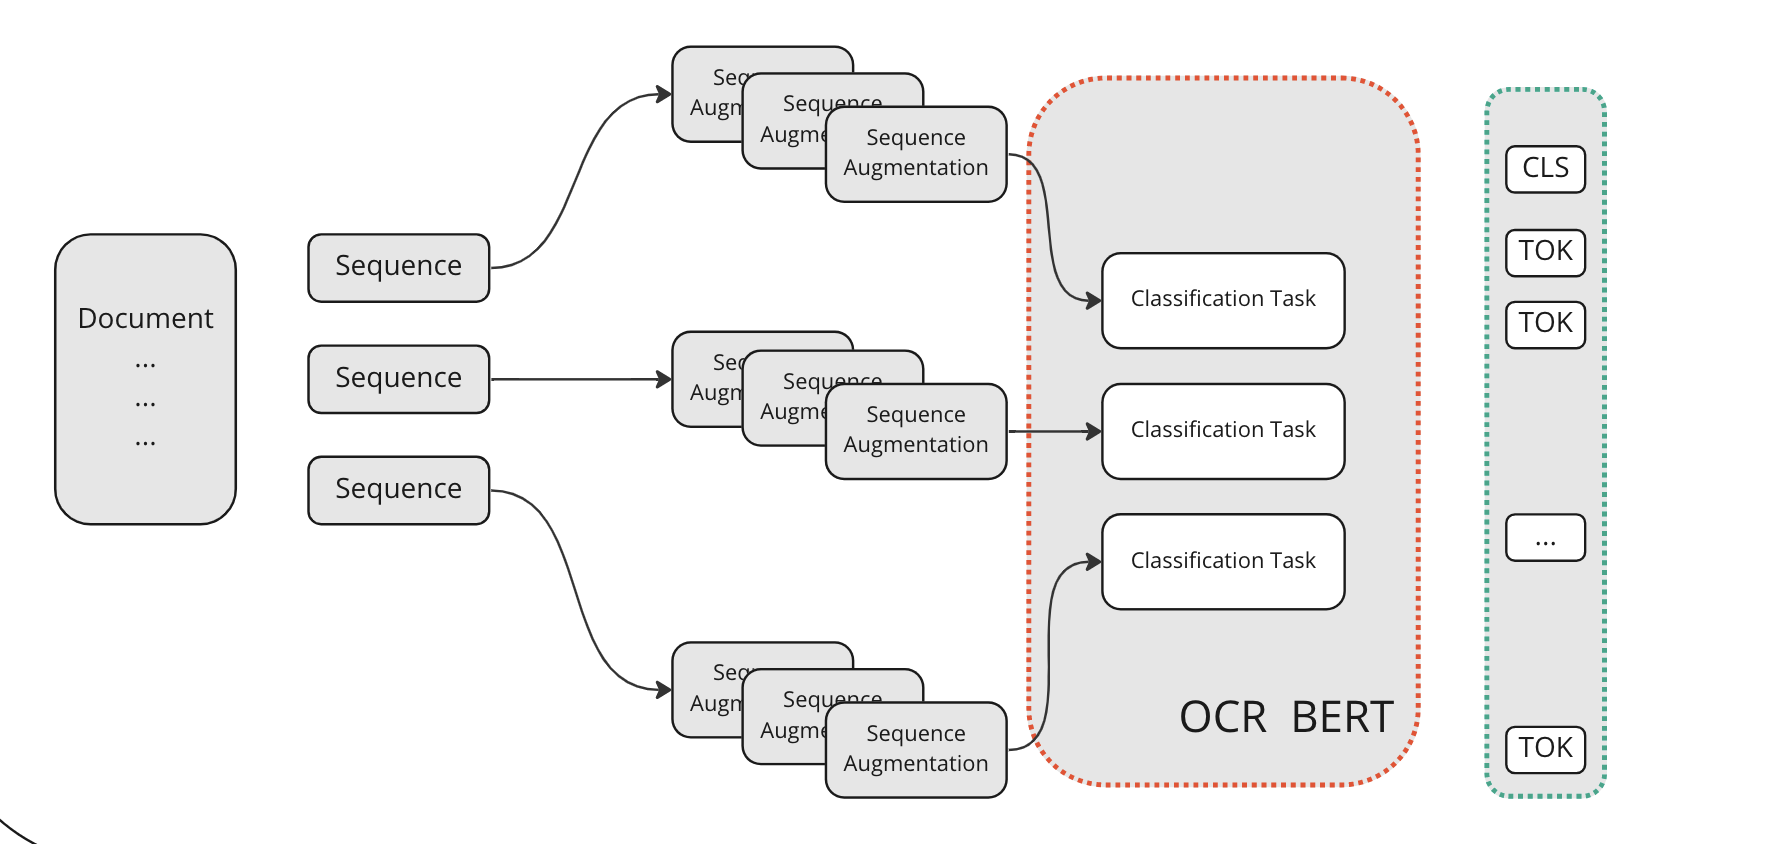
\includegraphics[scale=.5]{regularization}
    		\caption{Visual summary of regularizing classification token and embedding vector generated by Data Augmentation}
    		\label{fig:reg}
    	\end{figure}
	
 
 Embedding spaces when measuring similarity can be interpreted as a global set of documents $D$ where each kernel $K$ can be a subset of a specific set of documents $d_n$ or a global kernel of all documents $D$, where D is expressed as a a collection of documents $D=[d_{0}, d_{1}, ...,d_{n}]$ and each kernel K is expressed as a specified inner product of each dimension of  $D$ such that $K(x,y)=\phi(x)\cdot \phi(y)\ {}$. Here the mapping of each document for embedding observation can be defined as the following theorem:

\begin{theorem}
Let \(D\), be a sequence of unique documents with many to one mapping of extracted text items \(t\) expressed as $D=\{d_i \mapsto \{(t_j:[t_{aug,k]})\}\}$
where granularity is observed as: \\ 
$d_i$ is the unique number of documents \\
$t_j$ is the number of true lines extracted in each document \\ 
$t_k$ is the number of permuted data points in reference to $t_j$ \\ 
\end{theorem}


\begin{theorem}
Let each kernel $K$ can be a subset of a specific set of documents $d_n$ or a global kernel of all documents $D$, where D is expressed as a a collection of documents $D=[d_{0}, d_{1}, ...,d_{n}]$ and each kernel K is expressed as a specified inner product of each dimension of  $D$ such that $K(x,y)=\phi(x)\cdot \phi(y)\ {}$ \\ 
\end{theorem}

Once generated by manipulating an OCR extraction pipeline, and the other generated by character substitution of a clinical tokenization corpus. The augmentation pipeline in the figure below illustrates the two parallel processes created to supply two dimensions of permutations. The first feature pipeline, notated in blue, illustrates the process of gray-scaling, normalization and image resolution augments. In order to generate noise reflecting cosmetic imperfection, the resolution factor is the dependent pre-processing component used to generate various images to be fed to the OCR engine. The second, uses the cleanest OCR run with a fully functional pre-processing pipeline in order minimize extract. Once extraction is complete, the plain text is segmented and substituted using word injection provided from a pre-trained BioClinical BERT language transformer in an effort to introduce both common language substitution and random character insertion commonly generated by the output of OCR engines. These permutations are then aggregated by document to match their respective ground truth sample to supply base BERT with enough augmentations to perform regularization on scanned documents to create a more distinctive embedding space.

    \graphicspath{{Images/}}
    	\begin{figure}[htp]
    		\centering
    		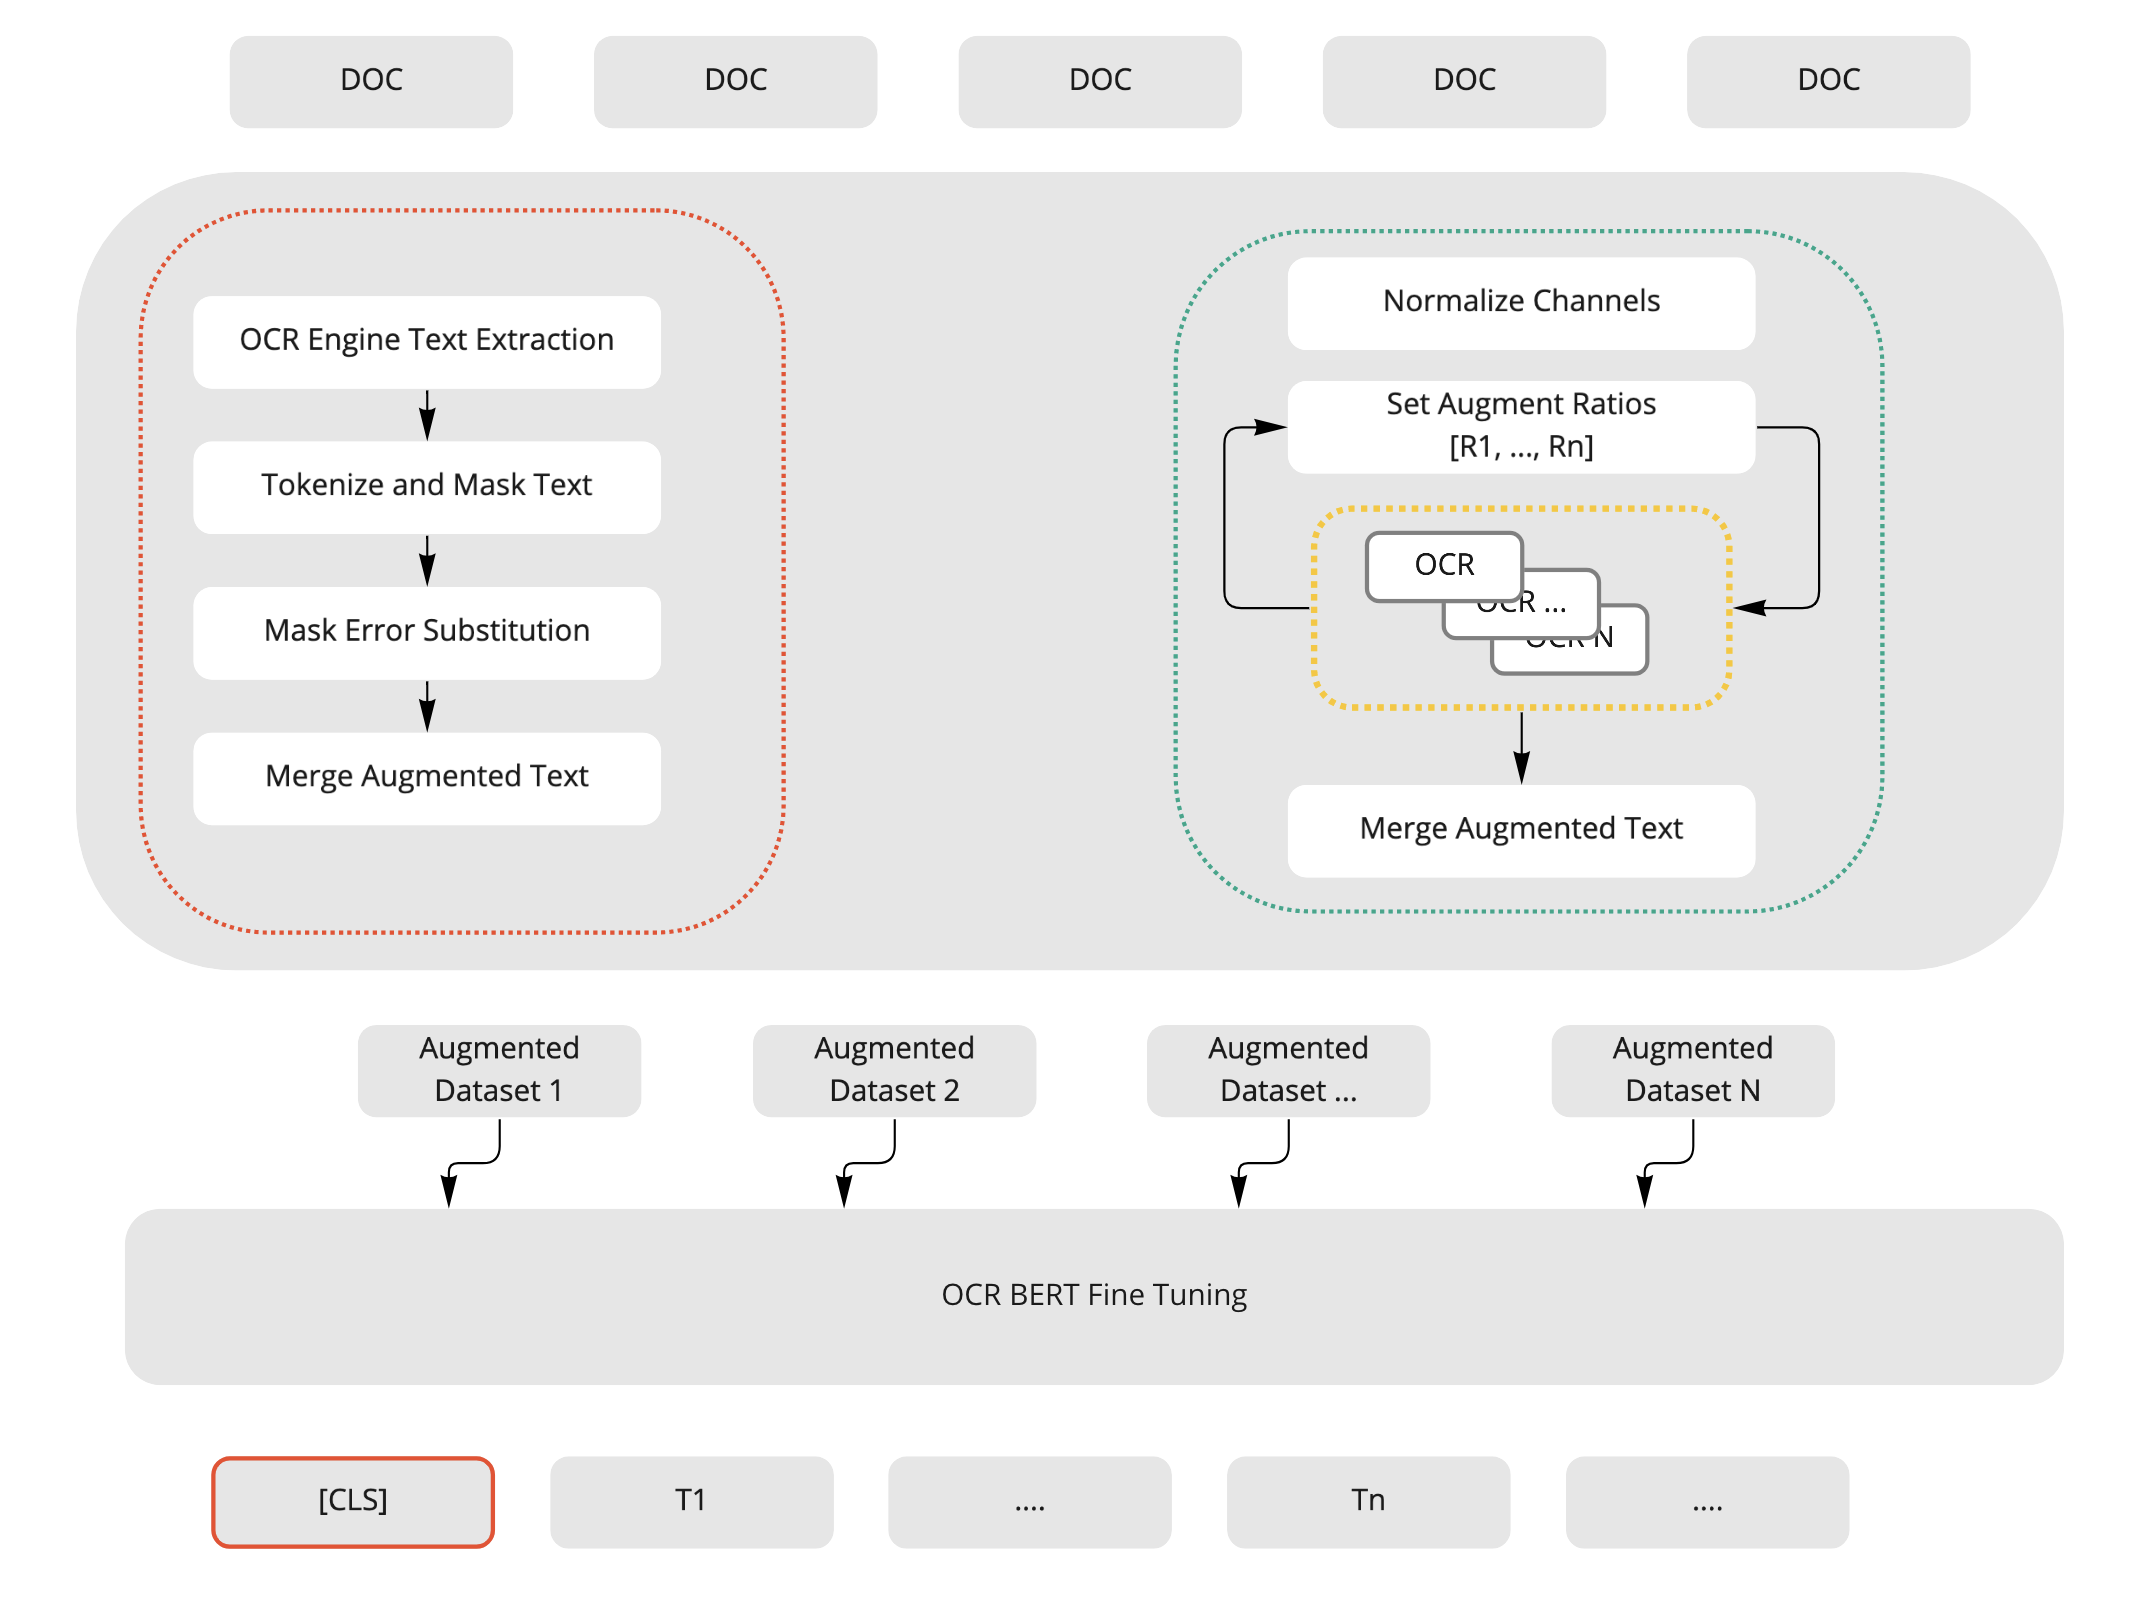
\includegraphics[scale=.25]{arch}
    		\caption{High level view of text and image augmentation strategy for fine tuning OCR BERT}
    		\label{fig:arch}
    	\end{figure}
	
    \subsection{Experimental Measurements}
    Given the two part hypothesis that introducing synthetic errors generated by an OCR engine, a task regularized embedding space will provide performance improvements for erroneous text extraction and act as a robust downstream feature extractor. Metrics for evaluating this study include the accuracy, harmonic mean of precision and recall in the form of an F1 score, and distribution of similarity within the various kernels. These measurements are supported and compared to the baseline transformer, BioClinical-BERT trained on the MIMIC-III discharge summaries. Our observations in more detail review: \\
        \textbf{Accuracy}: Given the classification task levels, specially annotation, we use accuracy as an illustration of improvement when regularizing the embedding space. However, this metric may not entirely illustrate drawbacks which moderate imbalance can present when extracting under represented information from sequences of text. \\
        \textbf{F1 Score} Because classification and annotation are two multi-class problems with varying levels of representation within their respective sub-memberships within the provided corpus a composite view of how each and class performs serves as a more detailed view of how each document groups regularization process performed each new task \\
        \textbf{Embedding Distribution and Similarity} Using synthetic error as a regularization technique in mapping class labels, erroneous data will have an influence on the distribution of the embedding space. We measure how well of a degree separation is being created within the high-dimensional generating embedding space using the cosine kernel. This will measure how well the embedding space itself can be used for downstream classification task in semi-supervised tasks. 
    
    \subsection{Baseline Model Selection}
    OCR BERT is a fine tuned implementation of the published medical corpus transformer BioClinical-bert published by Alsentzer et al. This model was selected over the pre-trained implementations BioMecial-BERT and BERT base due to the mixed language nature of the data this transformer was trained on; opposed to strictly clinical text, or plain Wikipedia articles. The novelty of this approach is not a variant BERT architecture, but the ability to fine tune and minimize the drawbacks of misclassification and data loss encountered by erroneous text extract engines for document annotation tasks in precision medicine. The modification is done at the embedding level instead of at the attention level.
    \subsection{Pre-Trained Model Initialization}
    Due to the baseline implementation of the model being the BioClinical-bert transformer, the weights and initialization can be reproduced by access the model via the Hugging Face artifact repository. Other considerations included base-bert-uncased and bio-bert. Both were presented as potential alternatives due to the specificity of the BioClinical-bert transformer and the effect said specificity would have on over generalizing a complete different application domain; Discharge summaries and clinical notes opposed to clinical treatment invoices. This disparity however, was ignored for the sake of leveraging the domain rich corpus the transformer was trained with to serve as an advantageous benchmark for feature extraction. 

\subsection{Dataset}
    \graphicspath{{Images/}}
	\begin{figure}[htp]
		\centering
		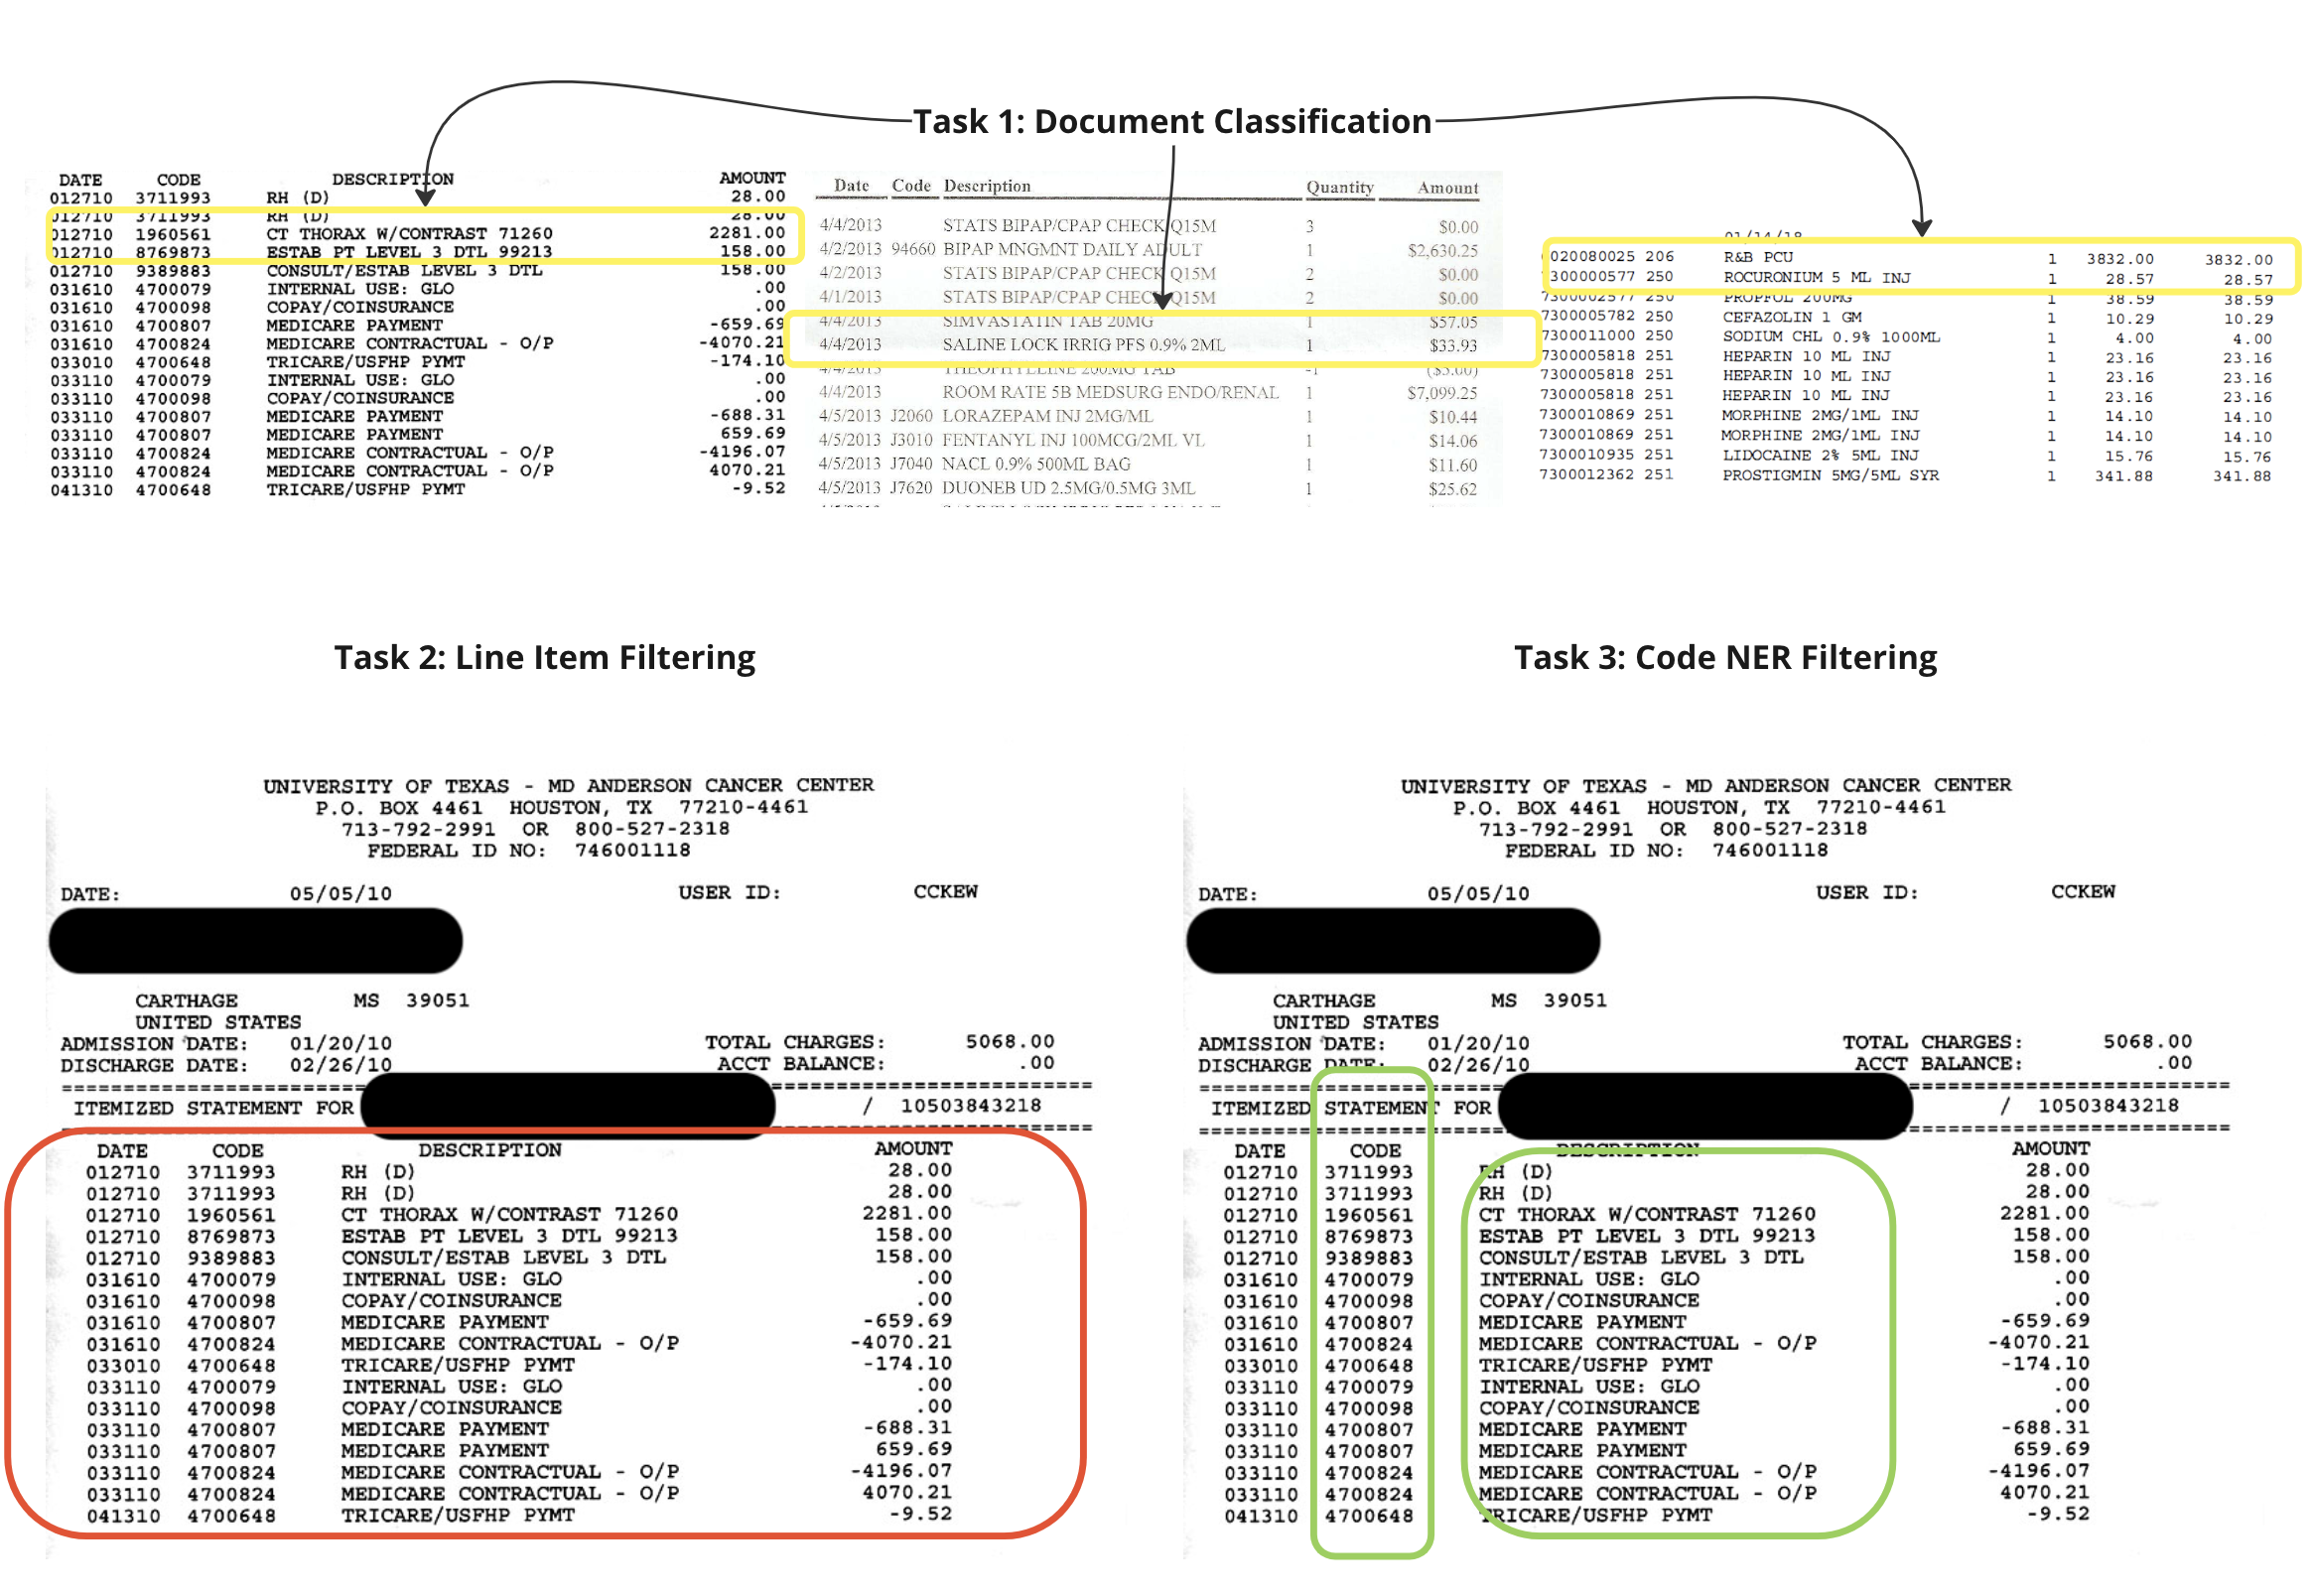
\includegraphics[scale=.3]{examples}
		\caption{Illustrating the classification and decision logic required to annotate documents of varying shapes and structure}
		\label{fig:examples}
	\end{figure}
Generally in practice, outside of a clinical lab setting the data generated for a patient or subject will have a human aspect to it, whether it be financial, communicative, or observatory. With that aspect to account for and the specialization of both English and Medical language transformers, there exists a realm between the two where mixed language introduces variation, noise, and error into most process(refers to creation of clinical Bert model and the authors tailored used cases around them). The data gathered for this experiment is in the form of plain text pdf and image data uploaded to the internet of released patient visits which include information such as services rendered, their item codes(ICD9/ICD10), and other relevant prescription and dosage information. Along with this information the presence of non-medical yet relevant data such as billing information, facility information, and invoice notes  are included in these documents; which intuitively add a level of complexity and bloat to the relevant clinical information a downstream task would ultimately want to extract and process. Along with the varying levels of inter document text representation, most invoices are specific in terms of literal document shape(the shape of the record, terms, and  language used) and reflect the facility or third party software that generated it. This challenge introduces the challenge of sub-class, class imbalance or large amounts of imbalance introduced by the large variance of similarity within an under-represented set of data. The purpose of leveraging this dataset is to present a real-world level of feasibility to a complex use case and to also test the sensitivity of the Clinical BERT embedding scores to create an abstraction between the mixed language and non-clinical text records present within the dataset. 



% \end{document}

%\graphicspath{{images}}
%\begin{figure}[htp]
%    \centering
%    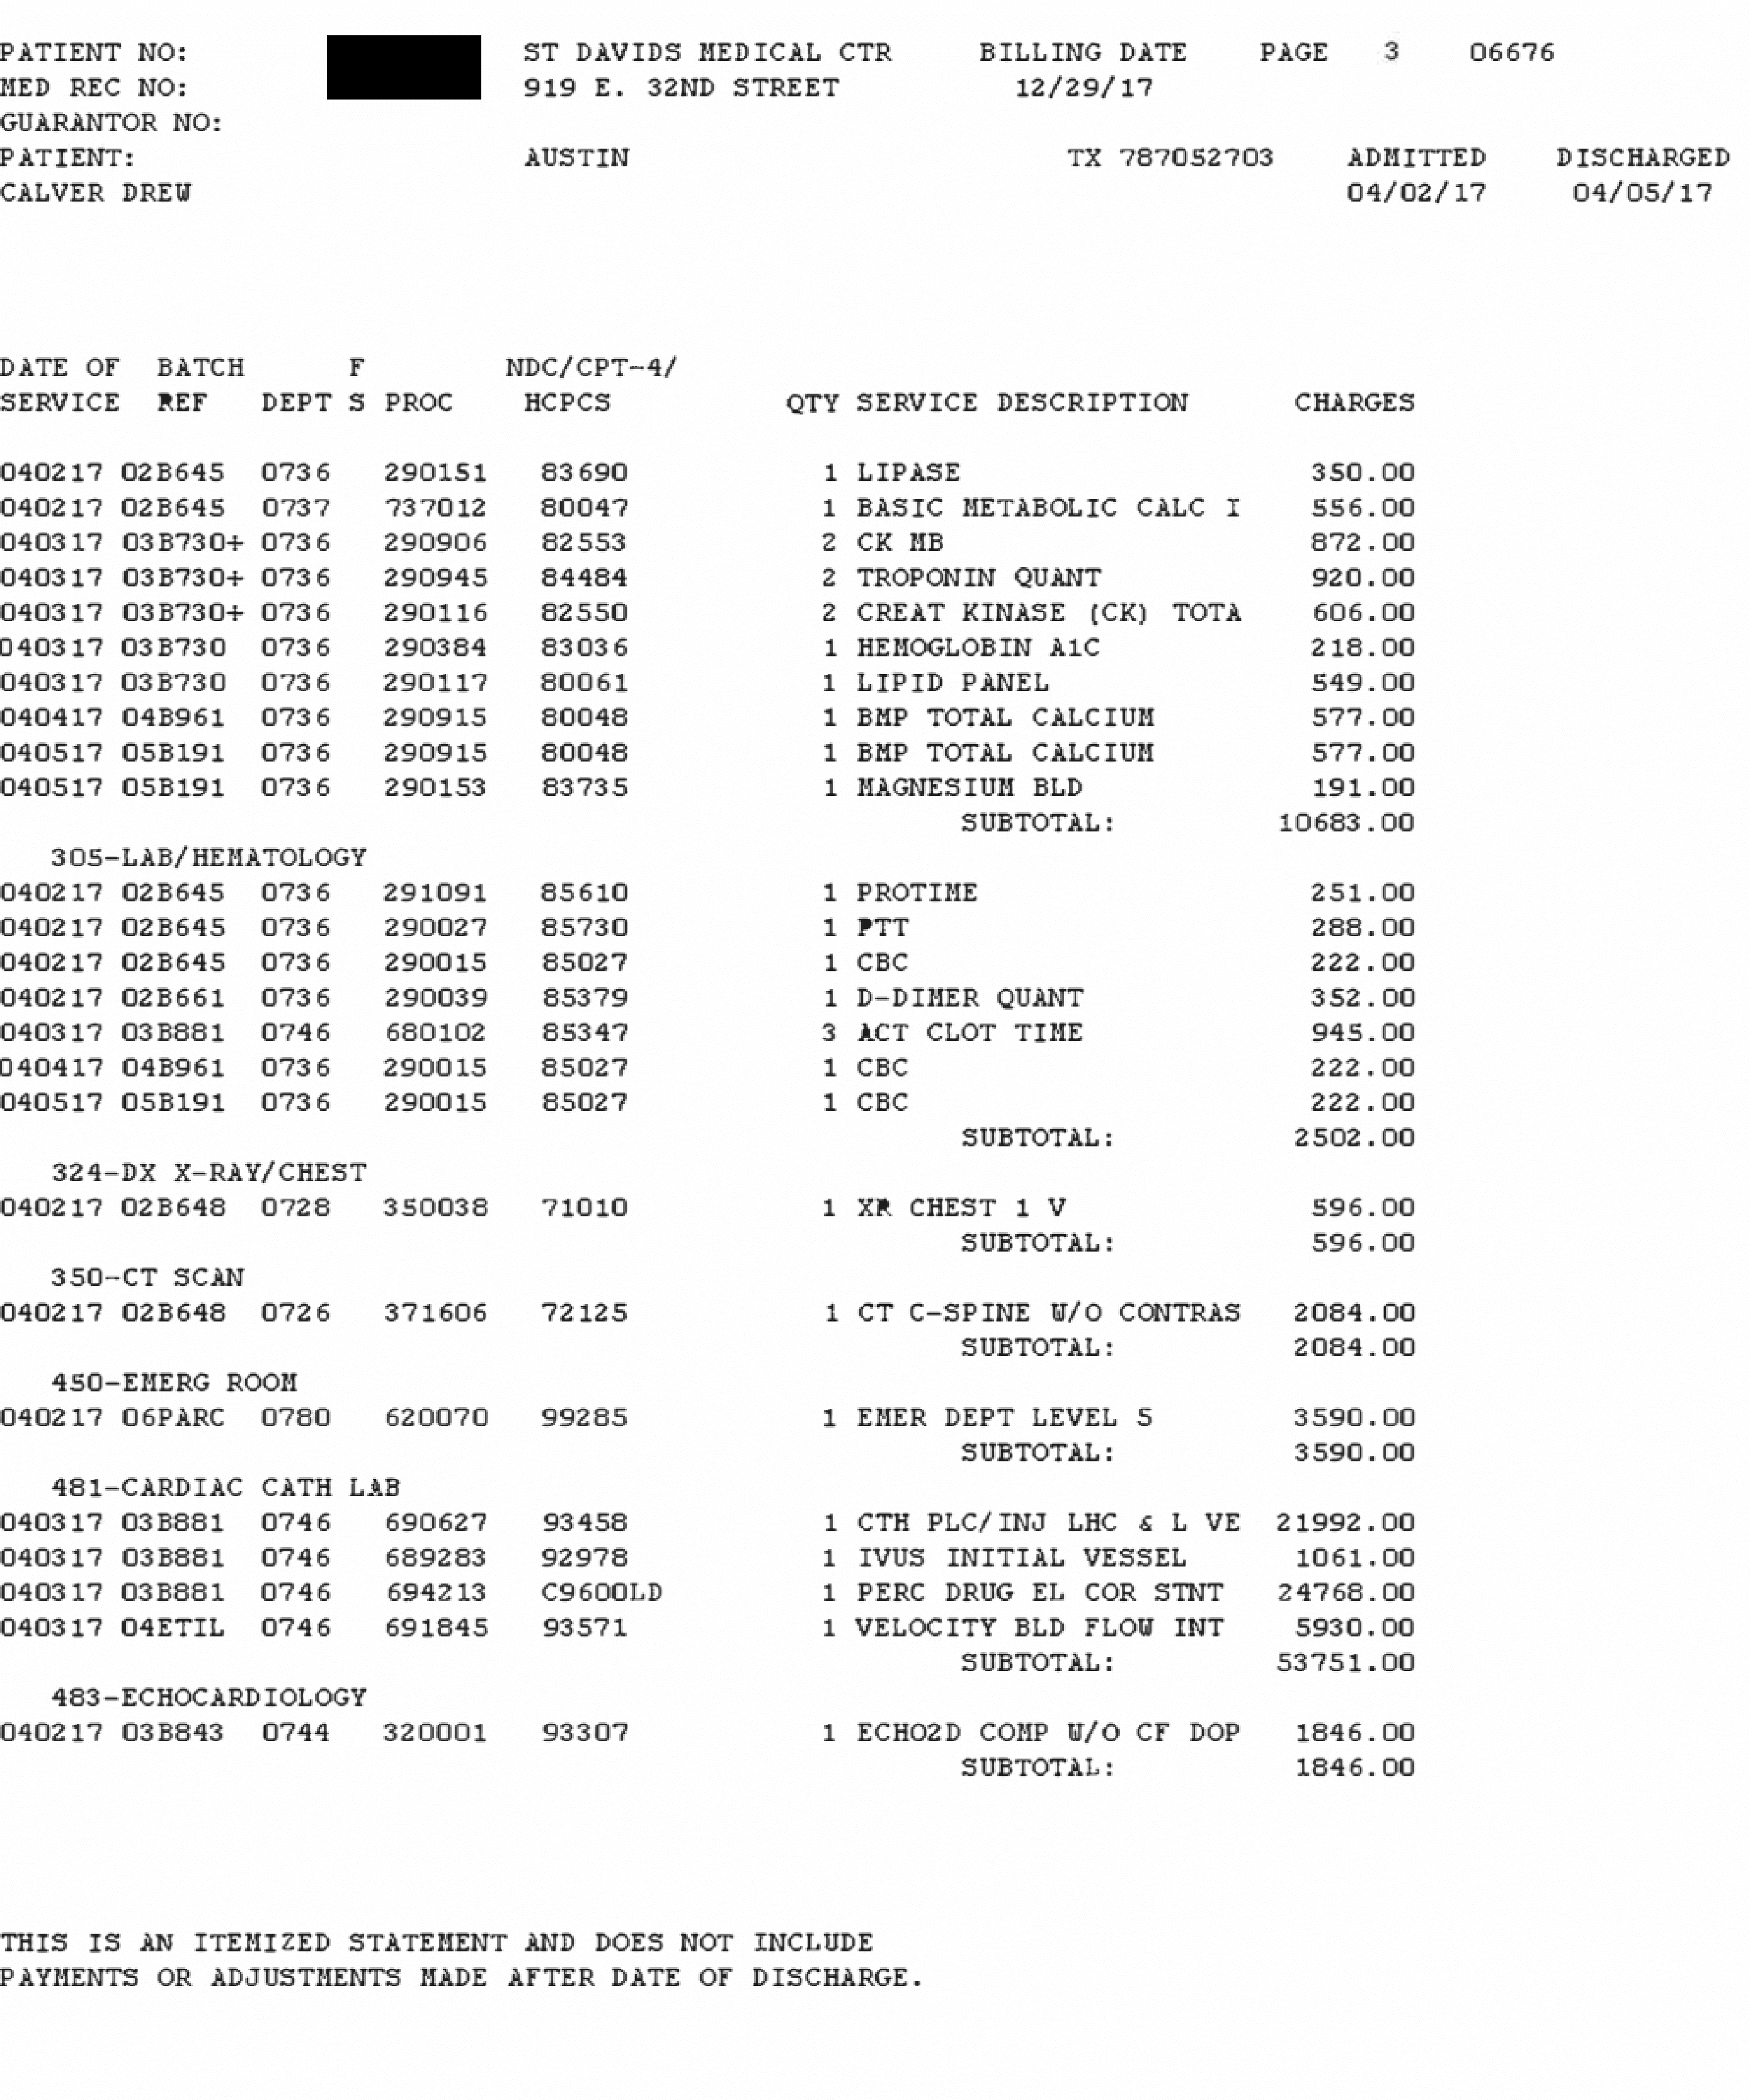
\includegraphics[scale=.10]{ncp-6-2}
%    \caption{Example of Semi Structured Medical Invoice}
%    \label{fig:ncp-6-2}
%\end{figure}
%
%\subsection{Data Augmentation}
%\subsubsection{Data Augmentation Algorithms}
%    \begin{algorithm}
%    \caption{Text Consistency Regularization Algorithm}
%    \label{alg:cap}
%    \begin{algorithmic}
%    \Require $n \geq 0$
%    \Ensure $aug=  f \circ g  $
%    \State $X \gets x$
%    \State $N \gets n$ \Comment{Where n is each unique document invoice shape}
%    \State $D \gets [d_0, d_1, ... d_n]$ \Comment{Where d is a unique document of type n}
%    \State $M = \sum_{n=1} ^{N} AUG_n \mapsto X_n$
%    \While{$N \neq 0$}
%        \If{Grain is "cosmetic"}
%            \State $AUG \gets CosmeticAUG(d) $\Comment{TODO: Define CosmeticAUG}
%        \ElsIf{Grain is "text"}
%            \State $AUG \gets SystemAUG(d) $\Comment{TODO: Define SystemAUG}
%        \EndIf
%       \EndWhile
%    \end{algorithmic}
%    \end{algorithm}
%
%\subsection{Model Fine Tuning}
%\subsection{Downstream Tasks}
%\subsubsection{Document Classification}
%\subsubsection{Document Line Level Annotation}
%\subsubsection{Regularized Feature Extraction}
%
%
%
%
\section{Results}
\subsection{OCR BERT Sequence Classification Fine Tuning}
\begin{table}[!ht]
    \centering
     \caption{OCR BERT Evaluation Metrics}
    \begin{tabular}{|l|l|l|l|l|l|}
    \hline
      ~ train loss & val loss & total acc & f1 d1 & f1 d2  & f1 d3 \\ \hline
       0.0555 & 0.034887 & 0.987559 & 0.9888849 & 0.97416744 & 0.99349892  \\ \hline
    \end{tabular}
\end{table}
\subsection{Observing the Change in Embedding Separability}
Using the embedding space created by applying OCR BERT and its respective parent token generator as a feature extraction pipeline, the following results are produced as displayed in Table 1. Unlike the a non-regularized transformer, the OCR-BERT implementation provided enough training points to introduce a higher degree of variance than its counterpart(see baseline standard deviation comparisons for each document $d_n$). The primary effect of the augmentation hypothesis was confirmed by the notion that introducing erroneous permutations of text would increase the overall quality of the embedding space due to the semi structured nature of each of the documents. A secondary effect is that the regularization acts as a high dimensional feature extraction mechanism that simplifies downstream classification efforts as noted in Figures 3 and 4; where a small subset of line items from each document class are clustered using a randomly initialized K-Means classifier to illustrate high dimensional separability. A counter argument to this approach and its results are the over specificity of the baseline model and its corpus used during the training process to establish the embedding space. In this case, measuring the performance of the transformation space by varying levels granularity with the training data is a potential outlet for further enhancing task specific fine-tuned transformers.

As a document classifier, OCR BERT
\begin{table}[!ht]
    \centering
     \caption{OCR BERT Embedding Space Distribution Summary}
    \begin{tabular}{|l|l|l|l|l|l|}
    \hline
        ~ & mean & std & min & max \\ \hline
        baseline\_{d1}  & 0.9226 & 0.0253 & 0.8062 & 0.9465 \\ \hline
        regularized\_{d1} & 0.9006 & 0.2137 & -0.044 & 0.9478 \\ \hline
        baseline\_{d2} & 0.9346 & 0.0204 & 0.875 & 0.9524 \\ \hline
        regularized\_{d2} & 0.8058 & 0.311 & -0.3736 & 0.896 \\ \hline
        baseline\_{d3} & 0.9387 & 0.0171 & 0.8938 & 0.9555 \\ \hline
        regularized\_{d3} & 0.9436 & 0.1614 & 0.0161 & 0.971 \\ \hline
        baseline\_{global} & 0.9268 & 0.0237 & 0.7935 & 0.9492 \\ \hline
        regularized\_{global} & 0.3117 & 0.1932 & -0.3799 & 0.4614 \\ \hline
    \end{tabular}
\end{table}
\subsection{Observing the Change in Embedding Quaility}
Given the probabilistic natured dataset such as the output of an OCR engine, creating an embedding space that accounts for the erroneous noise generated by the system exposed of the qualitative integrity of the embedding vectors generated. By comparing comparing the similarity scores of each document both local and global embedding spaces over generalized the text and created extremely tight embedding spaces with minimal separability as noted in Figure 3 and further explained by the increase in variance by each locally computed cosine kernel in Table 1. The comparison of locality to the baseline embedding space, was initially performed for document classification purposes, but later introduced the opportunity to extract pattern based tabular data from the documents. This assumption was encouraged by the fact the standard deviation and lower quartile of the embedding distribution has both increased; meaning we now had a simplified decision boundary to leverage.
\graphicspath{{images}}
\begin{figure}[htp]
    \center
    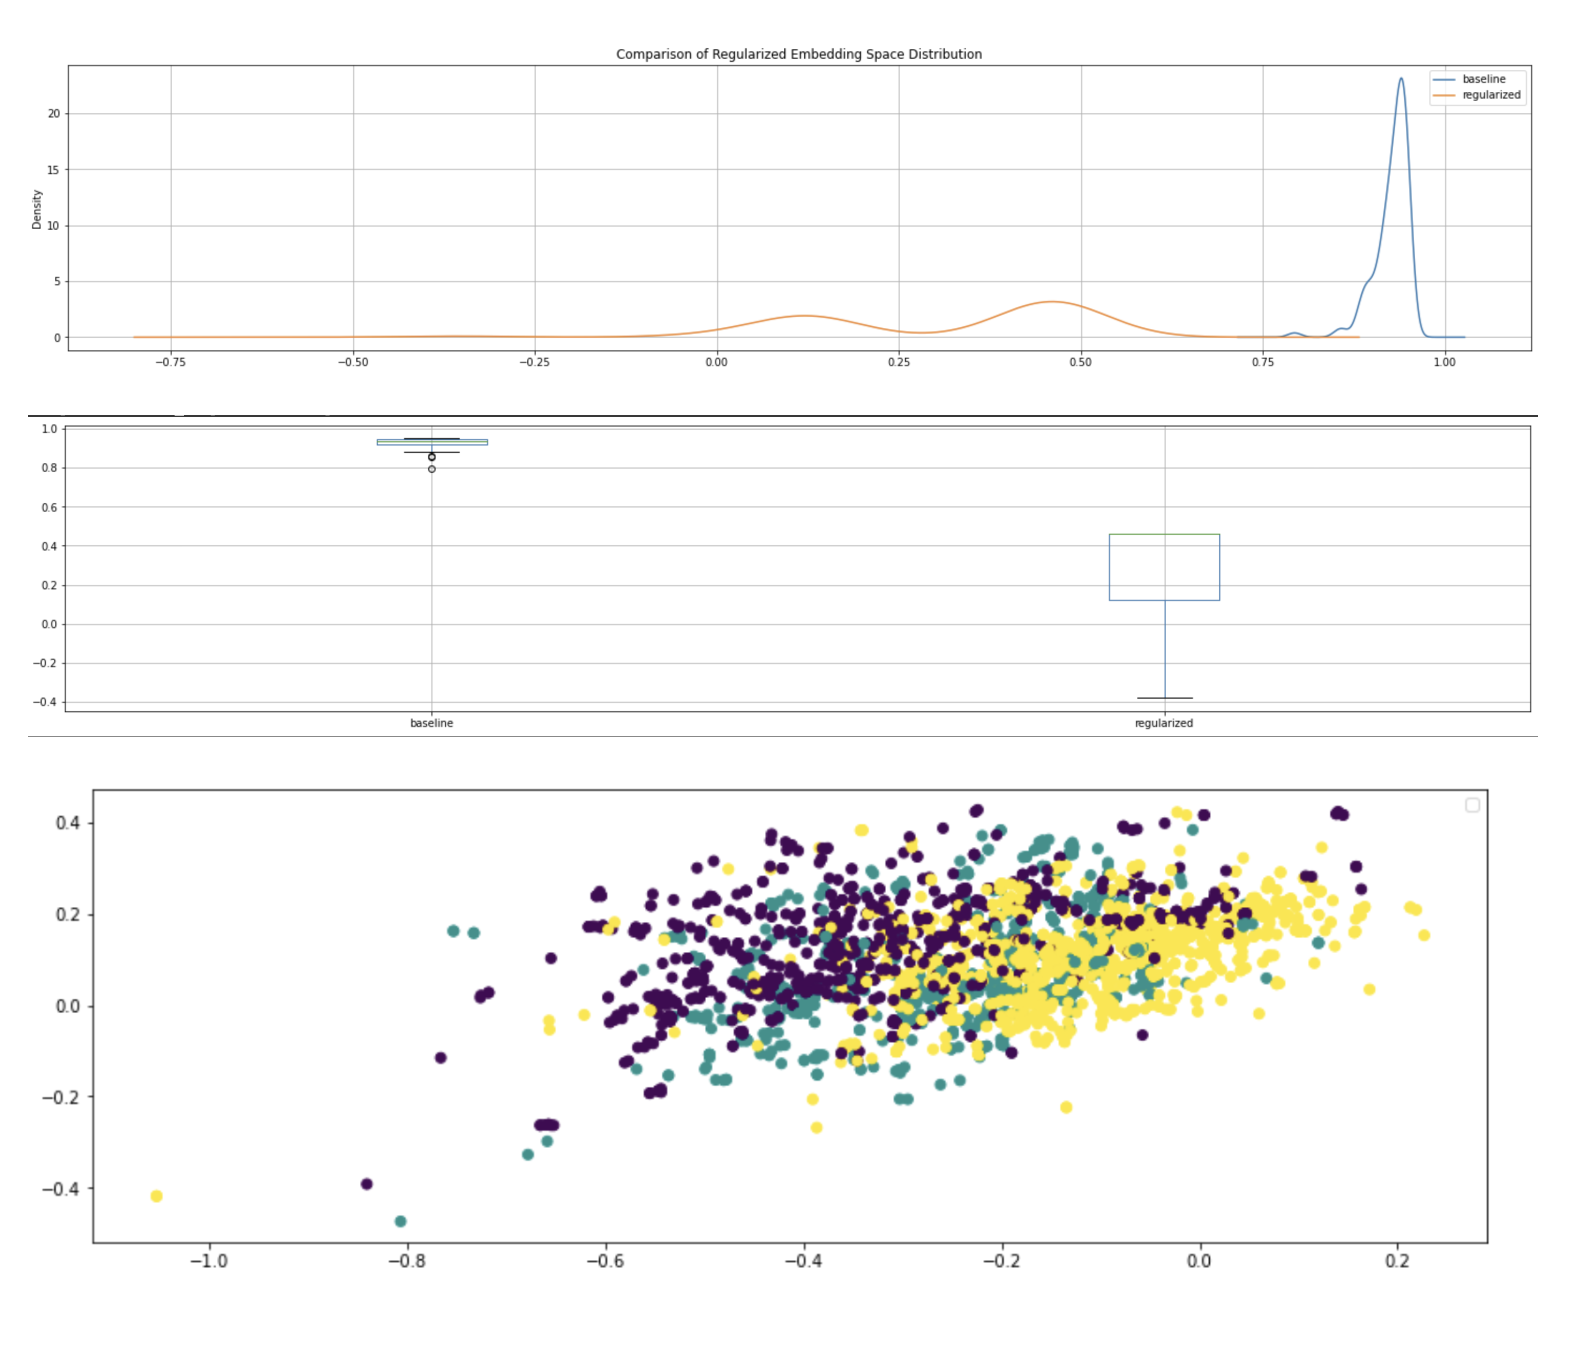
\includegraphics[scale=.33]{results1}
    \caption{Illustration of Embedding Generalization, by observing the change in distribution before and after data augmentation}
    \label{fig:res1} 
\end{figure}
\end{document}